\documentclass[english,compress]{beamer}
\usepackage{kloeckislides}
\nonstopmode

\usepackage[normalem]{ulem}
\usepackage{pifont}
\usepackage{ifthen}

\setbeamercolor{section in head/foot}{use=structure,bg=structure.fg!25!bg}
\defbeamertemplate*{footline}{split theme}
{%
  \leavevmode%
  \begin{beamercolorbox}[wd=.5\paperwidth,ht=2.5ex,dp=1.125ex]{section in head/foot}%
    \insertsectionnavigationhorizontal{\paperwidth}{\hskip0pt plus1filll}{}%
  \end{beamercolorbox}%
  %\begin{beamercolorbox}[wd=.5\paperwidth,ht=2.5ex,dp=1.125ex]{subsection in head/foot}%
    %\insertsubsectionnavigationhorizontal{.5\paperwidth}{}{\hskip0pt plus1filll}%
  %\end{beamercolorbox}%
}


%\useoutertheme[subsection=false]{miniframes}

\setbeamertemplate{frametitle}[default][center]

\AtBeginDocument{%
  {
    \usebeamercolor{section in head/foot}
  }
  
  \pgfdeclareverticalshading{beamer@headfade}{\paperwidth}
  {%
    color(0cm)=(bg);
    color(1.25cm)=(section in head/foot.bg)%
  }

  \setbeamercolor{section in head/foot}{bg=}
}

\addtoheadtemplate{\pgfuseshading{beamer@headfade}\vskip-1.25cm}{}

\beamertemplatedotitem

\setbeamercolor{section in head/foot}{parent=palette quaternary}
\setbeamercolor{subsection in head/foot}{parent=palette primary}

\setbeamercolor{author in head/foot}{parent=section in head/foot}
\setbeamercolor{title in head/foot}{parent=subsection in head/foot}



\AtBeginSection[] {
  \begin{frame}<beamer>
  \frametitle{Outline}
  \tableofcontents[sectionstyle=show/shaded,subsectionstyle=show/show/hide]
\end{frame}
}
\AtBeginSubsection[] {
  \begin{frame}<beamer>
  \frametitle{Outline}
  \tableofcontents[sectionstyle=show/shaded,subsectionstyle=show/shaded/hide]
\end{frame}
}

\newcommand{\technicality}[2]{%
  {\strut #1\\
    \begin{beamercolorbox}[sep=1mm]{block body}
      #2
    \end{beamercolorbox}
  }%
}

\lstset{
  language=C++,
  rangebeginprefix=//\ ,
  rangeendprefix=//\ ,
}

\def\weblink#1#2{\href{#1}{\color{blue}\underline{#2}}}

\definecolor{fetch}{RGB}{227,110,35}
\definecolor{alu}{RGB}{255,188,24}
\definecolor{context}{RGB}{132,146,175}

\usepackage{keystroke}

\setbeamertemplate{navigation symbols}{}

\def\hilite<#1>#2{\alt<#1>{\colorbox{blue!30}{#2}}{\colorbox{white}{#2}}%
}

\lstset{
  language=C++,
  rangebeginprefix=/*\ ,
  rangeendprefix=/*\ ,
}

\begin{document}
% {{{ front matter

\title{High-Performance Scientific Computing\\Lecture 9: Parallel Performance}

\date{MATH-GA 2011 / CSCI-GA 2945 $\cdot$ October 24, 2012}

\frame{\titlepage}

\begin{frame}{Today}
  \tableofcontents[hideallsubsections]
\end{frame}
% }}}
% -----------------------------------------------------------------------------
\begin{frame}{Bits and pieces}
  \begin{itemize}
    \item Don't have a project? Let's fix that \emph{very soon}
    \item HW5: soon
    \item HW6: due today
    \item Dec 5: Last day of regular class
    \item Dec 12: Legislative Day
    \item Dec 17/18/\textbf{19}: Project presentations
    \item Don't have grade reports for HW1\dots4? Talk to me
  \end{itemize}
\end{frame}
% -----------------------------------------------------------------------------
\section[Software]{Tool of the day: Shell scripting}
% -----------------------------------------------------------------------------
\begin{frame}{Shell scripting}
  \begin{center}
  \Huge Demo time
  \end{center}
\end{frame}
% -----------------------------------------------------------------------------
\begin{frame}{Shell scripting}
  \Large
  All you ever wanted to know about scripting:

  \begin{itemize}
    \item \url{http://tldp.org/LDP/abs/html/}
    \item \texttt{man bash}
  \end{itemize}
\end{frame}
% -----------------------------------------------------------------------------
\section{Single-thread performance}
% -----------------------------------------------------------------------------
\begin{frame}{Recap}
  Single-thread performance recap:
  \begin{itemize}
    \item CPU bits
      \subitem{Bus, Register File, ALU, Memory Interface, Machine
      language}
    \item Memory hierarchy
      \begin{itemize}
        \item Latency, bandwidth
        \item Caches: lines, associativity
        \item Locality, working set
      \end{itemize}
    \item Pipelines
      \begin{itemize}
        \item Dependencies
        \item Branch predictor
        \item Software pipelining, loop unrolling
      \end{itemize}
  \end{itemize}
\end{frame}
% -----------------------------------------------------------------------------
\subsection{How about actually doing work?}
% -----------------------------------------------------------------------------
\newcommand{\kayvoncredit}{
  \begin{tikzpicture}[overlay]
    \node [xshift=1cm,yshift=0.5cm]
      at (current page.south west)
      [font=\scriptsize,fill=gray!30,anchor=south west,opacity=0.5]
      {Credit: Kayvon Fatahalian (Stanford) };
  \end{tikzpicture}
}
\newcommand{\kayvonframe}[5]{

  \begin{frame}{#1}
    #4
    \begin{center}
    \includegraphics[viewport=#3,clip=true,page=#2,height=0.7\textheight]{kayvon-gpuarch.pdf}
    \end{center}
    \kayvoncredit
    #5
  \end{frame}
}
\begin{frame}{Remember SIMD?}
  \begin{columns}
    \column{0.5\textwidth}
      \only<1-2>{%
      \includegraphics[viewport=1.8in 3.8in 5.45in 6.25in,clip=true,page=19,width=\textwidth]{kayvon-gpuarch.pdf}\\[-0.5mm]
      \includegraphics[viewport=1.8in 1.35in 5.45in 3.8in,clip=true,page=19,width=\textwidth]{kayvon-gpuarch.pdf}
      }%
      \only<3>{%
      \includegraphics[viewport=1.8in 3.8in 5.45in 6.25in,clip=true,page=20,width=\textwidth]{kayvon-gpuarch.pdf}\\[-0.5mm]
      \includegraphics[viewport=1.8in 1.35in 5.45in 3.8in,clip=true,page=19,width=\textwidth]{kayvon-gpuarch.pdf}
      }%
      \only<4->{%
      \includegraphics[viewport=1.8in 3.8in 5.45in 6.25in,clip=true,page=20,width=\textwidth]{kayvon-gpuarch.pdf}\\[-0.5mm]
      \includegraphics[viewport=1.8in 1.35in 5.45in 3.8in,clip=true,page=20,width=\textwidth]{kayvon-gpuarch.pdf}
      }
    \column{0.5\textwidth}%
      \uncover<2->{%
        \textbf{GPU Idea \#2}

        \medskip
        Amortize cost/complexity of managing an instruction
        stream across many ALUs

        \medskip
        \large \textbf{$\rightarrow$ SIMD}
      }
  \end{columns}
  \kayvoncredit
  \uncover<5>{
    \begin{tikzpicture} [overlay]
      \node [above left=1cm of current page.south east,draw,drop shadow,fill=white,
       inner sep=5mm,thick]
        {
          Same principle works well on CPUs, too!
        } ;
    \end{tikzpicture}
  }
\end{frame}
% -----------------------------------------------------------------------------
\begin{frame}{Talking to SIMD}
  Ways of expressing SIMD:
  \begin{itemize}
    \item Not at all (\texttt{-ftree-vectorizer-verbose=2}, pray)
    \item ``Implicit'' (OpenCL workgroups)
    \item ``Explicit'' (many ways)
  \end{itemize}

  \bigskip
  OpenCL is also one of the saner ways of expressing
  \emph{explicit} vectorization.

  \emph{(even on the CPU)}

  \bigskip
  Other ways:
  \begin{itemize}
    \item ``Intrinsics'': \texttt{\_mm256\_hadd\_ps}
    \item GCC extensions
    \item \weblink{https://github.com/ispc/ispc}{ispc}
  \end{itemize}
\end{frame}
% -----------------------------------------------------------------------------
\begin{frame}{Floating point}
  \begin{center}
  \Huge CL vector demo
  \end{center}
\end{frame}
% }}}
% -----------------------------------------------------------------------------
\subsection[Compilers]{Compilers and what they do to your code}
% -----------------------------------------------------------------------------
\begin{frame}{Inside a compiler}
  \begin{center}
  \begin{tikzpicture}
  [every node/.style={draw,thick,fill=green!30,on chain,join,
  minimum height=4ex, minimum width=4cm},
  every join/.style={thick,->},
  chain default direction=going below,
  node distance=3mm,
  start chain
  ]
  \node {Preprocessor};
  \node {Parser};
  \node {\textbf<2->{Code generator}};
  \node {Assembler};
  \node {Linker};
  \node {(Dynamic Linker)};
  \end{tikzpicture}
  \end{center}
  \uncover<3->{
    \begin{tikzpicture} [overlay]
      \node [above left=1cm of current page.south east,draw,drop shadow,fill=white,
       inner sep=5mm,thick,text width=0.5\textwidth]
        {
          Two subsequent stages agree upon a data exchange format

          \bigskip
          ``Intermediate Representation''--
          often a little like assembly

          \bigskip
          Almost always more complicated: ``Passes'' include
          optimizers, \dots

          \url{http://llvm.org/demo/}
        } ;
    \end{tikzpicture}
  }
\end{frame}
% -----------------------------------------------------------------------------
\begin{frame}{Compilers and the register file}
  \begin{columns}
    \column{0.6\textwidth}
      Register allocator:
      \begin{itemize}
        \item Important
        \item Complicated
      \end{itemize}

      \medskip
      Failure: `Register Spill'

      \medskip
      Not dramatic on the CPU
      (L1 is fast)

      \medskip
      \emph{Very} dramatic on the GPU
    \column{0.4\textwidth}
    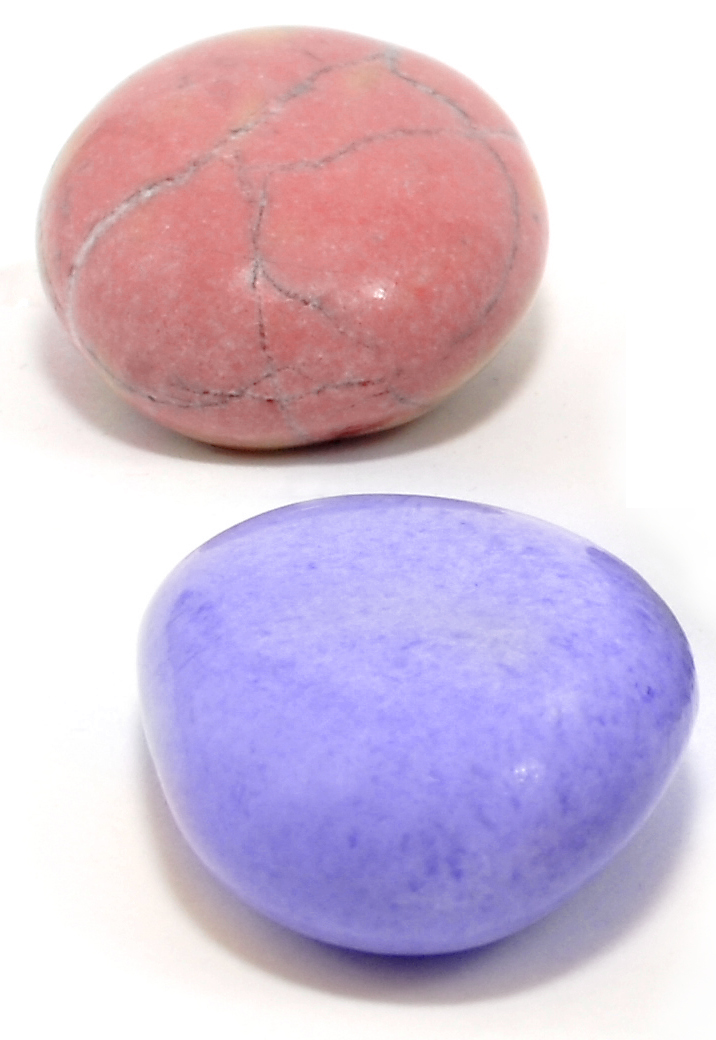
\includegraphics[width=\textwidth]{red-blue-pebble.jpeg}
  \end{columns}
  \uncover<2->{
    \begin{tikzpicture} [overlay]
      \node [above left=1cm of current page.south east,draw,drop shadow,fill=white,
       inner sep=5mm,thick, text width=0.5\textwidth]
        {
          Demo

          \only<2->{Registers most effective when data can be reused
            many times
          }
        } ;
    \end{tikzpicture}
  }
\end{frame}
\addimgcredit{Pebbles: sxc.hu/topfer}
% -----------------------------------------------------------------------------
\begin{frame}{Pointer aliasing}
  \begin{center}
  \Huge Pointer aliasing demo
  \end{center}
  \uncover<2->{
    \begin{tikzpicture} [overlay]
      \node [above left=1cm of current page.south east,draw,drop shadow,fill=white,
       inner sep=5mm,thick]
        {
          Not the only thing to go wrong with pointers\dots
        } ;
    \end{tikzpicture}
  }
\end{frame}
% -----------------------------------------------------------------------------
\begin{frame}{Alignment}
  \begin{columns}
    \column{0.45\textwidth}
    Match base address of:
    \begin{itemize}
      \item Single word: \texttt{double}, \texttt{float}
      \item SIMD vector
      \item Larger structure
    \end{itemize}
    \column{0.45\textwidth}
    To:
    \begin{itemize}
      \item Natural word size
      \item Vector size
      \item Cache line
    \end{itemize}
  \end{columns}

  \bigskip
  \begin{tikzpicture}[
    explanation/.style={right,inner xsep=0,text width=10cm}
    ]
    \foreach\addr in {0,1,...,34}
      \draw [fill=orange] 
        (0.25*\addr,0) coordinate (c\addr)
        rectangle +(0.25,0.25)
       coordinate [pos=0.5] (a\addr) ; 
    \draw (0.25*35,0) rectangle +(0.75,0.25)
       node [pos=0.5] { $\cdots$ }; 

    \foreach\addr in {0,16,32}
      \draw [ultra thick] (c\addr) -- +(0,0.25);

    \uncover<+->{
    \draw [snake=brace,thick,red] ($(c0) + (0,0.35)$) -- ($(c16) +(0,0.35)$) 
      node [pos=0.5,above] {Matched structure};
    }

    \coordinate (expl) at (0,-2.5) ;

    \uncover<+->{
      \begin{scope}[xshift=0cm,yshift=-1.5cm]
        \foreach\thread in {0,1,...,15}
          \draw [fill=gray!30] (0.25*\thread,0) rectangle +(0.25,0.25)
           coordinate [pos=0.5] (t\thread) ; 
      \end{scope}
    }

    \uncover<+>{
      \foreach\i in {0,1,...,15}
        \draw [thick,->] (t\i) -- (a\i) ;
      \node [explanation] at (expl)
      {
        {\color{green}OK}
      } ;
    }

    \uncover<+>{
      \node [explanation] at (expl)
      {
        {\color{red}``Bad''}
      } ;
    }

    \uncover<.>{
      \foreach\i in {0,1,...,15}
      {
        \pgfmathtruncatemacro{\addr}{5+\i}
        \draw [thick,->] (t\i) -- (a\addr) ;
      }
    }

    \uncover<+>{
      \foreach\i in {0,1,...,10}
      {
        \pgfmathtruncatemacro{\addr}{5+\i}
        \draw [thick,->] (t\i) -- (a\addr) ;
      }
      \foreach\i in {11,12,...,15}
      {
        \pgfmathtruncatemacro{\addr}{5+\i}
        \draw [thick,->,opacity=.1] (t\i) -- (a\addr) ;
      }
    }
    \uncover<+>{
      \foreach\i in {0,1,...,10}
      {
        \pgfmathtruncatemacro{\addr}{5+\i}
        \draw [thick,->,opacity=.1] (t\i) -- (a\addr) ;
      }
      \foreach\i in {11,12,...,15}
      {
        \pgfmathtruncatemacro{\addr}{5+\i}
        \draw [thick,->] (t\i) -- (a\addr) ;
      }
    }
  \end{tikzpicture}

  \uncover<+->{
    \begin{tikzpicture} [overlay]
      \node [above left=1cm of current page.south east,draw,drop shadow,fill=white,
       inner sep=5mm,thick, text width=0.9\textwidth]
        {
          Comes in two flavors:
          \begin{itemize}
            \item Actual alignment

              \texttt{malloc} $\rightarrow$ \texttt{posix\_memalign}
            \item Compiler-known alignment

              \texttt{float \_\_attribute\_\_ ((aligned (64))) *a}
          \end{itemize}

          \only<+->{
            \bigskip
            No difference on Sandy Bridge

            \bigskip
            More difference on other machines

            (e.g. AMD Opteron)
          }

          \only<+->{
            \bigskip
            Brief demo
          }
        } ;
    \end{tikzpicture}
  }
\end{frame}
% -----------------------------------------------------------------------------
\begin{frame}{Other compiler optimizations}
  More techniques:
  \begin{itemize}
    \item Inlining (see HW6)
    \item Unrolling
    \item Vectorization
  \end{itemize}

  \bigskip
  Many of these need tunable parameters. From where?
  \begin{itemize}
    \item \texttt{-march=native -mtune=native}
    \item Profile-Guided Optimization
  \end{itemize}
\end{frame}
% -----------------------------------------------------------------------------
\begin{frame}{From the horses' mouth}
  \begin{itemize}
    \item
      \weblink{http://support.amd.com/us/Processor_TechDocs/47414_15h_sw_opt_guide.pdf}{AMD Optimization Manual}
      \begin{itemize}
        \item Good source-level C part at the beginning
      \end{itemize}
    \item \weblink{http://www.intel.com/content/dam/doc/manual/64-ia-32-architectures-optimization-manual.pdf}{Intel Optimization Manual}
      \begin{itemize}
        \item Dual audience: Compiler writers, users
      \end{itemize}
  \end{itemize}

  \bigskip
  Grab bag of good practices:
  \begin{itemize}
    \item Use indices rather than pointers (easier to reason about)
    \item Extract common subexpressions
    \item Make functions static
    \item Use \texttt{const}
    \item Avoid store-to-load dependencies
  \end{itemize}
\end{frame}
% -----------------------------------------------------------------------------
\section{Multi-thread performance}
% -----------------------------------------------------------------------------
% {{{
\begin{frame}{Multi-thread performance}
  \begin{columns}
    \column{0.7\textwidth}

      Difference to single-thread?
      \pause

      \bigskip
      \textbf{Memory System} is (about) the only shared resource.

      \bigskip
      All `interesting' performance behavior of multiple threads
      has to do with that.
    \column{0.3\textwidth}
      \includegraphics[width=\textwidth]{memory.png}
  \end{columns}
\end{frame}
% -----------------------------------------------------------------------------
\subsection{Memory-related}
% -----------------------------------------------------------------------------
\begin{frame}{Multiple threads}
  \begin{center}
  \Huge Threads v. caches demo
  \end{center}
\end{frame}

\questionframe{}
\imagecreditslide

\end{document}
% vim: foldmethod=marker

